\section{Classi interne}
\subsection{Classi ed interfacce statiche innestate}
Le classi e le interfacce statiche innestate sono definite all'interno del corpo di una classeo di un'interfaccia e precedute da uno specificatore d'accesso (opzionale) e dalla parola chiave static.
\begin{lstlisting}
public class Persona {  
	public static class NomeAnagrafico { 
	   private String nome;    
	   private String cognome;    

	   public NomeAnagrafico(String n, String c) {
	         nome = n;      
	         cognome = c;    
	         }    
	         public String getNome() {
	               return nome;    
	               }    
	         public String getCognome() {
	               return cognome;    
	               }  
	    }  

	    private NomeAnagrafico nomeAnagrafico;  
	    public Persona(String n, String c) { 
	       nomeAnagrafico = new NomeAnagrafico(n, c);  
	       }  

	    public NomeAnagrafico getNomeAnagrafico() {
	        return nomeAnagrafico;  
	        }
	     }

\end{lstlisting}
La   classeNomeAnagrafico è interna, definita nel corpo della classe di   primo livello Persona. La compilazione del sorgente Persona.java porta alla nascita di due distinti bytecode: Persona.class e Persona\$NomeAnagrafico.java. La norma che fa corrispondere un bytecode ad ogni classe o interfaccia non è infranta.

Le classi statiche innestate fanno uso di quattro specificatori d'accesso:
\begin{itemize}
	\item \textbf{public}:  visibile ovunque mediante la notazione \textit{ClasseContenitrice.ClasseInterna};
	\item \textbf{private}: accessibile solo dal codice della classe che la contiene;
	\item \textbf{protected}: accessibile dal codice della classe che la contiene e dalle sue eventuali classi figlie, oltre che dal codice delle classi presenti nello stesso package;
	\item \textbf{Priva di specificatore}: disponibile solo all'interno del package che ospita la classe che la contiene.
	\end{itemize}
\subsection{Classi innestate non statiche}
Una \textbf{classe innestata} (o \textbf{classe interna} nel caso non sia dichiarata statica, o classe membro) non è altro che una classe definita all'interno di un'altra classe.
La limitazione delle classi interne statiche o delle interfacce statiche è che non possono invocare membri non statici della classe che li contiene. 
Esempio:
\begin{lstlisting}
public class Outer{
	public string messaggioOuter = "ciao";

	private void StampaMessaggio(){
	System.out.println(messaggioOuter);
	}

	public class Inner{
		public void Stampa(){
			StampaMessaggio();
		}
	}
}
\end{lstlisting}
La classe interna(Inner) ha accesso ai membri della classe esterna anche se dichiarati \textit{private}. Nell'esempio precedente la classe inner richiama il metodo StampaMessaggio() presente nella classe Outer.


\subsubsection{Proprietà}
\begin{itemize}
	\item Deve avere un identificatore differente dalla classe che la contiene;
	\item Per istanziare una classe interna al di fuori della classe in cui è definita bisogna seguire alcuni passi:
		\begin{itemize}
			\item istanziare la classe esterna in cui è dichiarata la classe interna : \textit{Outer outer = new Outer();}
			\item dichiarare l'oggetto che si vuole istanziare dalla classe interna tramite la classe interna: \textit{Outer.Inner oggettoInner;}
			\item istanziare l'oggetto della classe interna tramite l'oggetto istanziato dalla classe esterna: oggettoInner = out.new Inner();
		\end{itemize}
		\item ha accesso sia alle variabili d'istanza sia a quelle statiche delal classe in cui è contenuta;
		\item se viene dichiarata statica diventa automaticamente \textbf{top-level class}, quindi non potrà accedere alle variabili d'istanza nella classe che la contiene;
		\item solo se dichiarata statica può dichiarare membri statici;
		\item può essere dichiarata astratta;
		\item può utilizzare il reference this per accedere ai suoi membri interni (non a quelli della classe contenitrice);
		\item per accedere ai membri esterni a partire da una classe interna :\textit{NomeClasseEsterna.this.NomeMembroDellaClasseEsterna};
		\item se 2 classi hanno lo stesso membro verrà preso quello della classe interna;
	\end{itemize}

	\subsubsection{Quando usare le classi innestate}
	Potrebbe essere desiderabile creare una classe innestata solo in casi in cui ci sia una forte relazione tra la classe Inner e Outer. Per esempio una classe Auto potrebbe avere bisogno di una classe Meccanico che effettui delle riparazioni.
	La soluzione senza classi innestate potrebbe essere questa:
	\begin{lstlisting}
	public class AutoNoInner{
		private String statoMotore;
		private MeccanicoNoInner meccanico;

		public AutoNoInner(){
			meccanico = new MeccanicoNoInner(this);
		}

		public void setStatoMotore(String statoMotore){
			this.statoMotore = statoMotore;
		}
		public String getStatoMotore(){
			return statoMotore;
		}
	}

	pulic class MeccanicoNoInner{
		private AutoNoInner auto;

		public MeccanicoNoInner(AutoNoInner auto){
			this.auto = auto;
		}

		public void aggiustaMotore(){
			auto.setStatoMotore("buono");
		}
	}
	\end{lstlisting}

Invece la versione con le classi interne è la seguente:
\begin{lstlisting}
public class Auto{
	private String statoMotore;

	public class Meccanico{
		public void aggiustaMotore(){
		statoMotore = "buono";
		}
	}
}
\end{lstlisting}
Il lato negativo di utilizzare la classe interna è che se si vuole utilizzare la classe meccanico al di fuori della classe Auto, bisognerà sempre istanziare un'auto per istanziare un meccanico.

Altro esempio:
\begin{lstlisting}
class Outer {
	private int a;
	public Outer(int value) {
	a = value;
	}

	public class Inner {
		private int b;
		public Inner(int value) {
			b = a + value;
	}
		public void showValue() {
		System.out.println(b);
		}
	}

	public void printValue() {
		System.out.println(a);
	}
}

public class Main {
public static void main(...) {
	Outer o = new Outer(10);
	o.printValue();// stampa 10
	Outer.Inner i = o.new Inner(20);
	i.showValue();// stampa 30
	}
}
\end{lstlisting}
Notare che \textit{Inner i = new Inner(20)} non va bene perché le classi interne possono essere create solo se legate ad istanze di oggetti. Occorre quindi creare prima un oggetto della classe outer (fatto prima con new Outer(10)) e poi usare la sintassi Outer.Inner i = o.new Inner(20).

\subsection{Classi anonime}
Una classe anonima è una classe \textbf{locale} senza un nome assegnato, si tratta di una classe definita e instanziata un’unica volta attraverso una singola espressione caratterizzata da una versione estesa della sintassi dell’operatore new.
\begin{figure}[H]
\centering
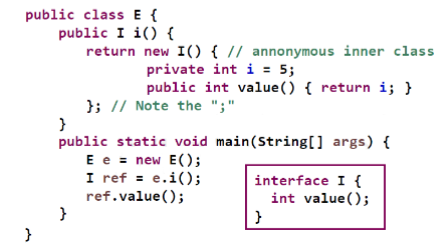
\includegraphics{images/anonime1}
\caption{Classe anonima\label{fig:UC3}}
\end{figure}
La definizione della classe è integrata nell’espressione di return o di dichiarazione di variabile, basta che ci sia l'operatore new. Una classe anonima è una notazione abbreviata per creare un semplice oggetto piccolo "inline" che racchiude del codice da eseguire. Di solito il tipo è una interfaccia.Nell’esempio sopra la classe è castata ad una interface; sarebbe equivalente a:
\begin{lstlisting}
class Anonima implements I { ... }; 

return new Anonima();
\end{lstlisting}
A differenza delle classi interne, una classe anonima richieda che:
\begin{itemize}
	\item al momento della dichiarazione della classe venga istanziato un suo oggetto;
	\item ci sia l'esistenza di una classe o di una superinterfaccia di cui sfrutterà il costruttore(solo virtualmente nel caso di un'interfaccia). Se una classe non ha nome non può avere un costruttore.
\end{itemize}
Se compiliamo una classe che contiene delle classi anonime verrano creati tanti file quante sono le classi anonime.
\begin{lstlisting}
public class Outer{
	private string messaggio = "Nella classe";

	/*Definizione della classe anonima e sua istanza*/
	ClasseAnonima ca = new ClasseAnonima(){
		@Override
		public void metodo(){
			System.out.println(messaggio + "anonima");
		}
	};

	/*superclasse della classe anonima*/
	public class ClasseAnonima{
		public void metodo(){
			System.out.println("Nella classe anonima");
		}
	}
}
\end{lstlisting}
La classe anonima dell'esempio usa il reference ca di tipo ClasseAnonima per referenziare un oggetto della sua sottoclasse anonima, e implicitamente come tutte le sottoclassi chiama sempre il costruttore della superclasse.

Una classe anonima viene dichiarata con lo scopo do fare override di uno  più metodi della classe che la estende. Se infatti nell'esempio di prima avessimo definito un nuovo metodo (non ereditato) nella classe anonima, non saremmo stati in grado di invocarlo senza un reference del tipo della classe anonima (che però non può esistere).
\begin{lstlisting}


	/*Definizione della classe anonima e sua istanza*/
	ClasseAnonima ca = new ClasseAnonima(){
		@Override
		public void metodo(){
			System.out.println(messaggio + "anonima");
		}
	};

	public void metodoNonInvocabile(){
	System.out.println("Per una classe anonima non esistono 
	reference. Impossibile chiamare questo metodo!");
	}
}
\end{lstlisting}